\section{Example\-Frame\-Listener Class Reference}
\label{classExampleFrameListener}\index{ExampleFrameListener@{ExampleFrameListener}}
{\tt \#include $<$Example\-Frame\-Listener.h$>$}

Inheritance diagram for Example\-Frame\-Listener::\begin{figure}[H]
\begin{center}
\leavevmode
\includegraphics[height=2cm]{classExampleFrameListener}
\end{center}
\end{figure}
Collaboration diagram for Example\-Frame\-Listener:\begin{figure}[H]
\begin{center}
\leavevmode
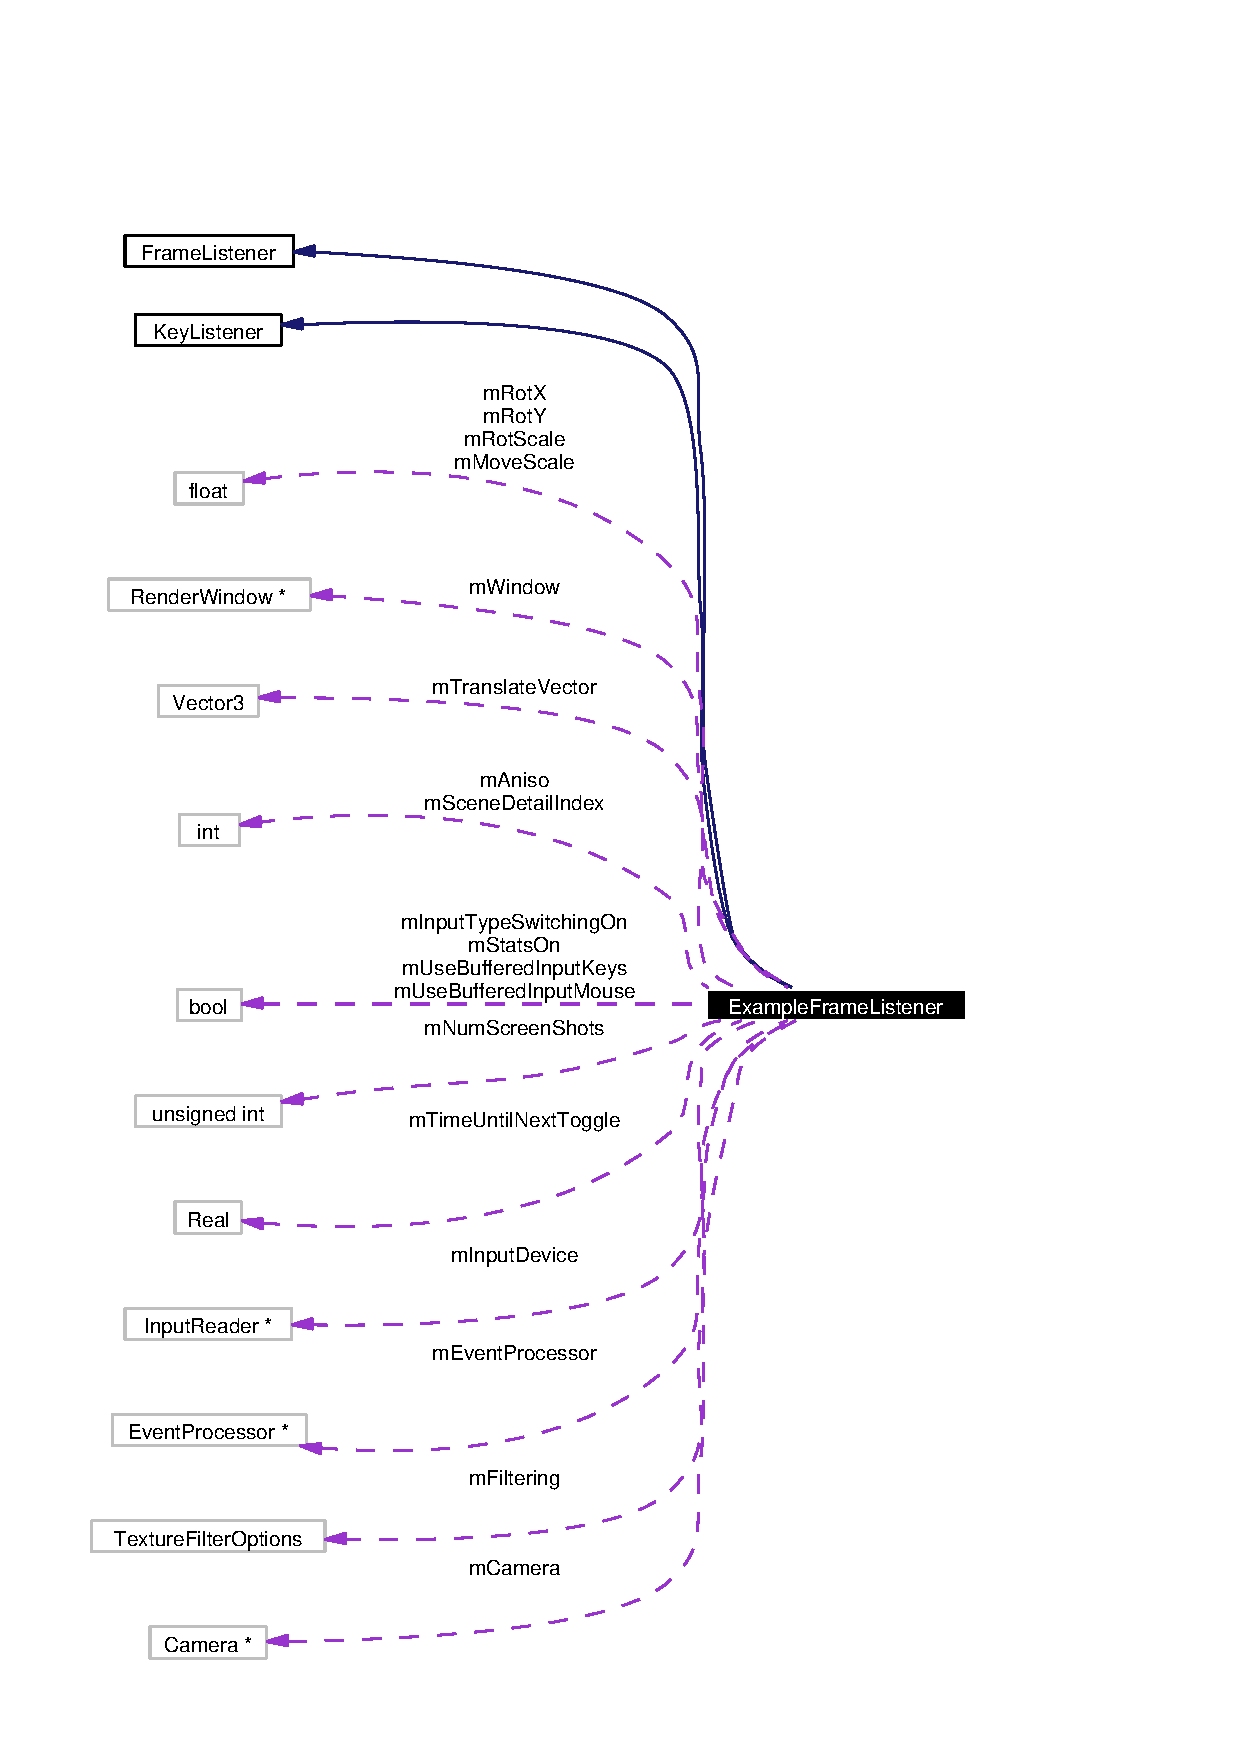
\includegraphics[width=236pt]{classExampleFrameListener__coll__graph}
\end{center}
\end{figure}
\subsection*{Public Member Functions}
\begin{CompactItemize}
\item 
{\bf Example\-Frame\-Listener} (Render\-Window $\ast$win, Camera $\ast$cam, bool use\-Buffered\-Input\-Keys=false, bool use\-Buffered\-Input\-Mouse=false)
\item 
virtual {\bf $\sim$Example\-Frame\-Listener} ()
\item 
virtual bool {\bf process\-Unbuffered\-Key\-Input} (const Frame\-Event \&evt)
\item 
bool {\bf process\-Unbuffered\-Mouse\-Input} (const Frame\-Event \&evt)
\item 
void {\bf move\-Camera} ()
\item 
void {\bf show\-Debug\-Overlay} (bool show)
\item 
bool {\bf frame\-Started} (const Frame\-Event \&evt)
\item 
bool {\bf frame\-Ended} (const Frame\-Event \&evt)
\item 
void {\bf switch\-Mouse\-Mode} ()
\item 
void {\bf switch\-Key\-Mode} ()
\item 
void {\bf key\-Clicked} (Key\-Event $\ast$e)
\item 
void {\bf key\-Pressed} (Key\-Event $\ast$e)
\item 
void {\bf key\-Released} (Key\-Event $\ast$e)
\end{CompactItemize}
\subsection*{Protected Attributes}
\begin{CompactItemize}
\item 
Event\-Processor $\ast$ {\bf m\-Event\-Processor}
\item 
Input\-Reader $\ast$ {\bf m\-Input\-Device}
\item 
Camera $\ast$ {\bf m\-Camera}
\item 
Vector3 {\bf m\-Translate\-Vector}
\item 
Render\-Window $\ast$ {\bf m\-Window}
\item 
bool {\bf m\-Stats\-On}
\item 
bool {\bf m\-Use\-Buffered\-Input\-Keys}
\item 
bool {\bf m\-Use\-Buffered\-Input\-Mouse}
\item 
bool {\bf m\-Input\-Type\-Switching\-On}
\item 
unsigned int {\bf m\-Num\-Screen\-Shots}
\item 
float {\bf m\-Move\-Scale}
\item 
float {\bf m\-Rot\-Scale}
\item 
Real {\bf m\-Time\-Until\-Next\-Toggle}
\item 
float {\bf m\-Rot\-X}
\item 
float {\bf m\-Rot\-Y}
\item 
Texture\-Filter\-Options {\bf m\-Filtering}
\item 
int {\bf m\-Aniso}
\end{CompactItemize}
\subsection*{Private Member Functions}
\begin{CompactItemize}
\item 
void {\bf update\-Stats} (void)
\end{CompactItemize}
\subsection*{Private Attributes}
\begin{CompactItemize}
\item 
int {\bf m\-Scene\-Detail\-Index}
\end{CompactItemize}


\subsection{Constructor \& Destructor Documentation}
\index{ExampleFrameListener@{Example\-Frame\-Listener}!ExampleFrameListener@{ExampleFrameListener}}
\index{ExampleFrameListener@{ExampleFrameListener}!ExampleFrameListener@{Example\-Frame\-Listener}}
\subsubsection{\setlength{\rightskip}{0pt plus 5cm}Example\-Frame\-Listener::Example\-Frame\-Listener (Render\-Window $\ast$ {\em win}, Camera $\ast$ {\em cam}, bool {\em use\-Buffered\-Input\-Keys} = false, bool {\em use\-Buffered\-Input\-Mouse} = false)\hspace{0.3cm}{\tt  [inline]}}\label{classExampleFrameListener_a0}


\index{ExampleFrameListener@{Example\-Frame\-Listener}!~ExampleFrameListener@{$\sim$ExampleFrameListener}}
\index{~ExampleFrameListener@{$\sim$ExampleFrameListener}!ExampleFrameListener@{Example\-Frame\-Listener}}
\subsubsection{\setlength{\rightskip}{0pt plus 5cm}virtual Example\-Frame\-Listener::$\sim${\bf Example\-Frame\-Listener} ()\hspace{0.3cm}{\tt  [inline, virtual]}}\label{classExampleFrameListener_a1}




\subsection{Member Function Documentation}
\index{ExampleFrameListener@{Example\-Frame\-Listener}!frameEnded@{frameEnded}}
\index{frameEnded@{frameEnded}!ExampleFrameListener@{Example\-Frame\-Listener}}
\subsubsection{\setlength{\rightskip}{0pt plus 5cm}bool Example\-Frame\-Listener::frame\-Ended (const Frame\-Event \& {\em evt})\hspace{0.3cm}{\tt  [inline]}}\label{classExampleFrameListener_a7}


\index{ExampleFrameListener@{Example\-Frame\-Listener}!frameStarted@{frameStarted}}
\index{frameStarted@{frameStarted}!ExampleFrameListener@{Example\-Frame\-Listener}}
\subsubsection{\setlength{\rightskip}{0pt plus 5cm}bool Example\-Frame\-Listener::frame\-Started (const Frame\-Event \& {\em evt})\hspace{0.3cm}{\tt  [inline]}}\label{classExampleFrameListener_a6}


\index{ExampleFrameListener@{Example\-Frame\-Listener}!keyClicked@{keyClicked}}
\index{keyClicked@{keyClicked}!ExampleFrameListener@{Example\-Frame\-Listener}}
\subsubsection{\setlength{\rightskip}{0pt plus 5cm}void Example\-Frame\-Listener::key\-Clicked (Key\-Event $\ast$ {\em e})\hspace{0.3cm}{\tt  [inline]}}\label{classExampleFrameListener_a10}


\index{ExampleFrameListener@{Example\-Frame\-Listener}!keyPressed@{keyPressed}}
\index{keyPressed@{keyPressed}!ExampleFrameListener@{Example\-Frame\-Listener}}
\subsubsection{\setlength{\rightskip}{0pt plus 5cm}void Example\-Frame\-Listener::key\-Pressed (Key\-Event $\ast$ {\em e})\hspace{0.3cm}{\tt  [inline]}}\label{classExampleFrameListener_a11}


\index{ExampleFrameListener@{Example\-Frame\-Listener}!keyReleased@{keyReleased}}
\index{keyReleased@{keyReleased}!ExampleFrameListener@{Example\-Frame\-Listener}}
\subsubsection{\setlength{\rightskip}{0pt plus 5cm}void Example\-Frame\-Listener::key\-Released (Key\-Event $\ast$ {\em e})\hspace{0.3cm}{\tt  [inline]}}\label{classExampleFrameListener_a12}


\index{ExampleFrameListener@{Example\-Frame\-Listener}!moveCamera@{moveCamera}}
\index{moveCamera@{moveCamera}!ExampleFrameListener@{Example\-Frame\-Listener}}
\subsubsection{\setlength{\rightskip}{0pt plus 5cm}void Example\-Frame\-Listener::move\-Camera ()\hspace{0.3cm}{\tt  [inline]}}\label{classExampleFrameListener_a4}


\index{ExampleFrameListener@{Example\-Frame\-Listener}!processUnbufferedKeyInput@{processUnbufferedKeyInput}}
\index{processUnbufferedKeyInput@{processUnbufferedKeyInput}!ExampleFrameListener@{Example\-Frame\-Listener}}
\subsubsection{\setlength{\rightskip}{0pt plus 5cm}virtual bool Example\-Frame\-Listener::process\-Unbuffered\-Key\-Input (const Frame\-Event \& {\em evt})\hspace{0.3cm}{\tt  [inline, virtual]}}\label{classExampleFrameListener_a2}


\index{ExampleFrameListener@{Example\-Frame\-Listener}!processUnbufferedMouseInput@{processUnbufferedMouseInput}}
\index{processUnbufferedMouseInput@{processUnbufferedMouseInput}!ExampleFrameListener@{Example\-Frame\-Listener}}
\subsubsection{\setlength{\rightskip}{0pt plus 5cm}bool Example\-Frame\-Listener::process\-Unbuffered\-Mouse\-Input (const Frame\-Event \& {\em evt})\hspace{0.3cm}{\tt  [inline]}}\label{classExampleFrameListener_a3}


\index{ExampleFrameListener@{Example\-Frame\-Listener}!showDebugOverlay@{showDebugOverlay}}
\index{showDebugOverlay@{showDebugOverlay}!ExampleFrameListener@{Example\-Frame\-Listener}}
\subsubsection{\setlength{\rightskip}{0pt plus 5cm}void Example\-Frame\-Listener::show\-Debug\-Overlay (bool {\em show})\hspace{0.3cm}{\tt  [inline]}}\label{classExampleFrameListener_a5}


\index{ExampleFrameListener@{Example\-Frame\-Listener}!switchKeyMode@{switchKeyMode}}
\index{switchKeyMode@{switchKeyMode}!ExampleFrameListener@{Example\-Frame\-Listener}}
\subsubsection{\setlength{\rightskip}{0pt plus 5cm}void Example\-Frame\-Listener::switch\-Key\-Mode ()\hspace{0.3cm}{\tt  [inline]}}\label{classExampleFrameListener_a9}


\index{ExampleFrameListener@{Example\-Frame\-Listener}!switchMouseMode@{switchMouseMode}}
\index{switchMouseMode@{switchMouseMode}!ExampleFrameListener@{Example\-Frame\-Listener}}
\subsubsection{\setlength{\rightskip}{0pt plus 5cm}void Example\-Frame\-Listener::switch\-Mouse\-Mode ()\hspace{0.3cm}{\tt  [inline]}}\label{classExampleFrameListener_a8}


\index{ExampleFrameListener@{Example\-Frame\-Listener}!updateStats@{updateStats}}
\index{updateStats@{updateStats}!ExampleFrameListener@{Example\-Frame\-Listener}}
\subsubsection{\setlength{\rightskip}{0pt plus 5cm}void Example\-Frame\-Listener::update\-Stats (void)\hspace{0.3cm}{\tt  [inline, private]}}\label{classExampleFrameListener_d0}




\subsection{Member Data Documentation}
\index{ExampleFrameListener@{Example\-Frame\-Listener}!mAniso@{mAniso}}
\index{mAniso@{mAniso}!ExampleFrameListener@{Example\-Frame\-Listener}}
\subsubsection{\setlength{\rightskip}{0pt plus 5cm}int {\bf Example\-Frame\-Listener::m\-Aniso}\hspace{0.3cm}{\tt  [protected]}}\label{classExampleFrameListener_p16}


\index{ExampleFrameListener@{Example\-Frame\-Listener}!mCamera@{mCamera}}
\index{mCamera@{mCamera}!ExampleFrameListener@{Example\-Frame\-Listener}}
\subsubsection{\setlength{\rightskip}{0pt plus 5cm}Camera$\ast$ {\bf Example\-Frame\-Listener::m\-Camera}\hspace{0.3cm}{\tt  [protected]}}\label{classExampleFrameListener_p2}


\index{ExampleFrameListener@{Example\-Frame\-Listener}!mEventProcessor@{mEventProcessor}}
\index{mEventProcessor@{mEventProcessor}!ExampleFrameListener@{Example\-Frame\-Listener}}
\subsubsection{\setlength{\rightskip}{0pt plus 5cm}Event\-Processor$\ast$ {\bf Example\-Frame\-Listener::m\-Event\-Processor}\hspace{0.3cm}{\tt  [protected]}}\label{classExampleFrameListener_p0}


\index{ExampleFrameListener@{Example\-Frame\-Listener}!mFiltering@{mFiltering}}
\index{mFiltering@{mFiltering}!ExampleFrameListener@{Example\-Frame\-Listener}}
\subsubsection{\setlength{\rightskip}{0pt plus 5cm}Texture\-Filter\-Options {\bf Example\-Frame\-Listener::m\-Filtering}\hspace{0.3cm}{\tt  [protected]}}\label{classExampleFrameListener_p15}


\index{ExampleFrameListener@{Example\-Frame\-Listener}!mInputDevice@{mInputDevice}}
\index{mInputDevice@{mInputDevice}!ExampleFrameListener@{Example\-Frame\-Listener}}
\subsubsection{\setlength{\rightskip}{0pt plus 5cm}Input\-Reader$\ast$ {\bf Example\-Frame\-Listener::m\-Input\-Device}\hspace{0.3cm}{\tt  [protected]}}\label{classExampleFrameListener_p1}


\index{ExampleFrameListener@{Example\-Frame\-Listener}!mInputTypeSwitchingOn@{mInputTypeSwitchingOn}}
\index{mInputTypeSwitchingOn@{mInputTypeSwitchingOn}!ExampleFrameListener@{Example\-Frame\-Listener}}
\subsubsection{\setlength{\rightskip}{0pt plus 5cm}bool {\bf Example\-Frame\-Listener::m\-Input\-Type\-Switching\-On}\hspace{0.3cm}{\tt  [protected]}}\label{classExampleFrameListener_p8}


\index{ExampleFrameListener@{Example\-Frame\-Listener}!mMoveScale@{mMoveScale}}
\index{mMoveScale@{mMoveScale}!ExampleFrameListener@{Example\-Frame\-Listener}}
\subsubsection{\setlength{\rightskip}{0pt plus 5cm}float {\bf Example\-Frame\-Listener::m\-Move\-Scale}\hspace{0.3cm}{\tt  [protected]}}\label{classExampleFrameListener_p10}


\index{ExampleFrameListener@{Example\-Frame\-Listener}!mNumScreenShots@{mNumScreenShots}}
\index{mNumScreenShots@{mNumScreenShots}!ExampleFrameListener@{Example\-Frame\-Listener}}
\subsubsection{\setlength{\rightskip}{0pt plus 5cm}unsigned int {\bf Example\-Frame\-Listener::m\-Num\-Screen\-Shots}\hspace{0.3cm}{\tt  [protected]}}\label{classExampleFrameListener_p9}


\index{ExampleFrameListener@{Example\-Frame\-Listener}!mRotScale@{mRotScale}}
\index{mRotScale@{mRotScale}!ExampleFrameListener@{Example\-Frame\-Listener}}
\subsubsection{\setlength{\rightskip}{0pt plus 5cm}float {\bf Example\-Frame\-Listener::m\-Rot\-Scale}\hspace{0.3cm}{\tt  [protected]}}\label{classExampleFrameListener_p11}


\index{ExampleFrameListener@{Example\-Frame\-Listener}!mRotX@{mRotX}}
\index{mRotX@{mRotX}!ExampleFrameListener@{Example\-Frame\-Listener}}
\subsubsection{\setlength{\rightskip}{0pt plus 5cm}float {\bf Example\-Frame\-Listener::m\-Rot\-X}\hspace{0.3cm}{\tt  [protected]}}\label{classExampleFrameListener_p13}


\index{ExampleFrameListener@{Example\-Frame\-Listener}!mRotY@{mRotY}}
\index{mRotY@{mRotY}!ExampleFrameListener@{Example\-Frame\-Listener}}
\subsubsection{\setlength{\rightskip}{0pt plus 5cm}float {\bf Example\-Frame\-Listener::m\-Rot\-Y}\hspace{0.3cm}{\tt  [protected]}}\label{classExampleFrameListener_p14}


\index{ExampleFrameListener@{Example\-Frame\-Listener}!mSceneDetailIndex@{mSceneDetailIndex}}
\index{mSceneDetailIndex@{mSceneDetailIndex}!ExampleFrameListener@{Example\-Frame\-Listener}}
\subsubsection{\setlength{\rightskip}{0pt plus 5cm}int {\bf Example\-Frame\-Listener::m\-Scene\-Detail\-Index}\hspace{0.3cm}{\tt  [private]}}\label{classExampleFrameListener_r0}


\index{ExampleFrameListener@{Example\-Frame\-Listener}!mStatsOn@{mStatsOn}}
\index{mStatsOn@{mStatsOn}!ExampleFrameListener@{Example\-Frame\-Listener}}
\subsubsection{\setlength{\rightskip}{0pt plus 5cm}bool {\bf Example\-Frame\-Listener::m\-Stats\-On}\hspace{0.3cm}{\tt  [protected]}}\label{classExampleFrameListener_p5}


\index{ExampleFrameListener@{Example\-Frame\-Listener}!mTimeUntilNextToggle@{mTimeUntilNextToggle}}
\index{mTimeUntilNextToggle@{mTimeUntilNextToggle}!ExampleFrameListener@{Example\-Frame\-Listener}}
\subsubsection{\setlength{\rightskip}{0pt plus 5cm}Real {\bf Example\-Frame\-Listener::m\-Time\-Until\-Next\-Toggle}\hspace{0.3cm}{\tt  [protected]}}\label{classExampleFrameListener_p12}


\index{ExampleFrameListener@{Example\-Frame\-Listener}!mTranslateVector@{mTranslateVector}}
\index{mTranslateVector@{mTranslateVector}!ExampleFrameListener@{Example\-Frame\-Listener}}
\subsubsection{\setlength{\rightskip}{0pt plus 5cm}Vector3 {\bf Example\-Frame\-Listener::m\-Translate\-Vector}\hspace{0.3cm}{\tt  [protected]}}\label{classExampleFrameListener_p3}


\index{ExampleFrameListener@{Example\-Frame\-Listener}!mUseBufferedInputKeys@{mUseBufferedInputKeys}}
\index{mUseBufferedInputKeys@{mUseBufferedInputKeys}!ExampleFrameListener@{Example\-Frame\-Listener}}
\subsubsection{\setlength{\rightskip}{0pt plus 5cm}bool {\bf Example\-Frame\-Listener::m\-Use\-Buffered\-Input\-Keys}\hspace{0.3cm}{\tt  [protected]}}\label{classExampleFrameListener_p6}


\index{ExampleFrameListener@{Example\-Frame\-Listener}!mUseBufferedInputMouse@{mUseBufferedInputMouse}}
\index{mUseBufferedInputMouse@{mUseBufferedInputMouse}!ExampleFrameListener@{Example\-Frame\-Listener}}
\subsubsection{\setlength{\rightskip}{0pt plus 5cm}bool {\bf Example\-Frame\-Listener::m\-Use\-Buffered\-Input\-Mouse}\hspace{0.3cm}{\tt  [protected]}}\label{classExampleFrameListener_p7}


\index{ExampleFrameListener@{Example\-Frame\-Listener}!mWindow@{mWindow}}
\index{mWindow@{mWindow}!ExampleFrameListener@{Example\-Frame\-Listener}}
\subsubsection{\setlength{\rightskip}{0pt plus 5cm}Render\-Window$\ast$ {\bf Example\-Frame\-Listener::m\-Window}\hspace{0.3cm}{\tt  [protected]}}\label{classExampleFrameListener_p4}




The documentation for this class was generated from the following file:\begin{CompactItemize}
\item 
src/graphics/{\bf Example\-Frame\-Listener.h}\end{CompactItemize}
